\section{Supplementary Figures}
\begin{suppfigure}[h!]
    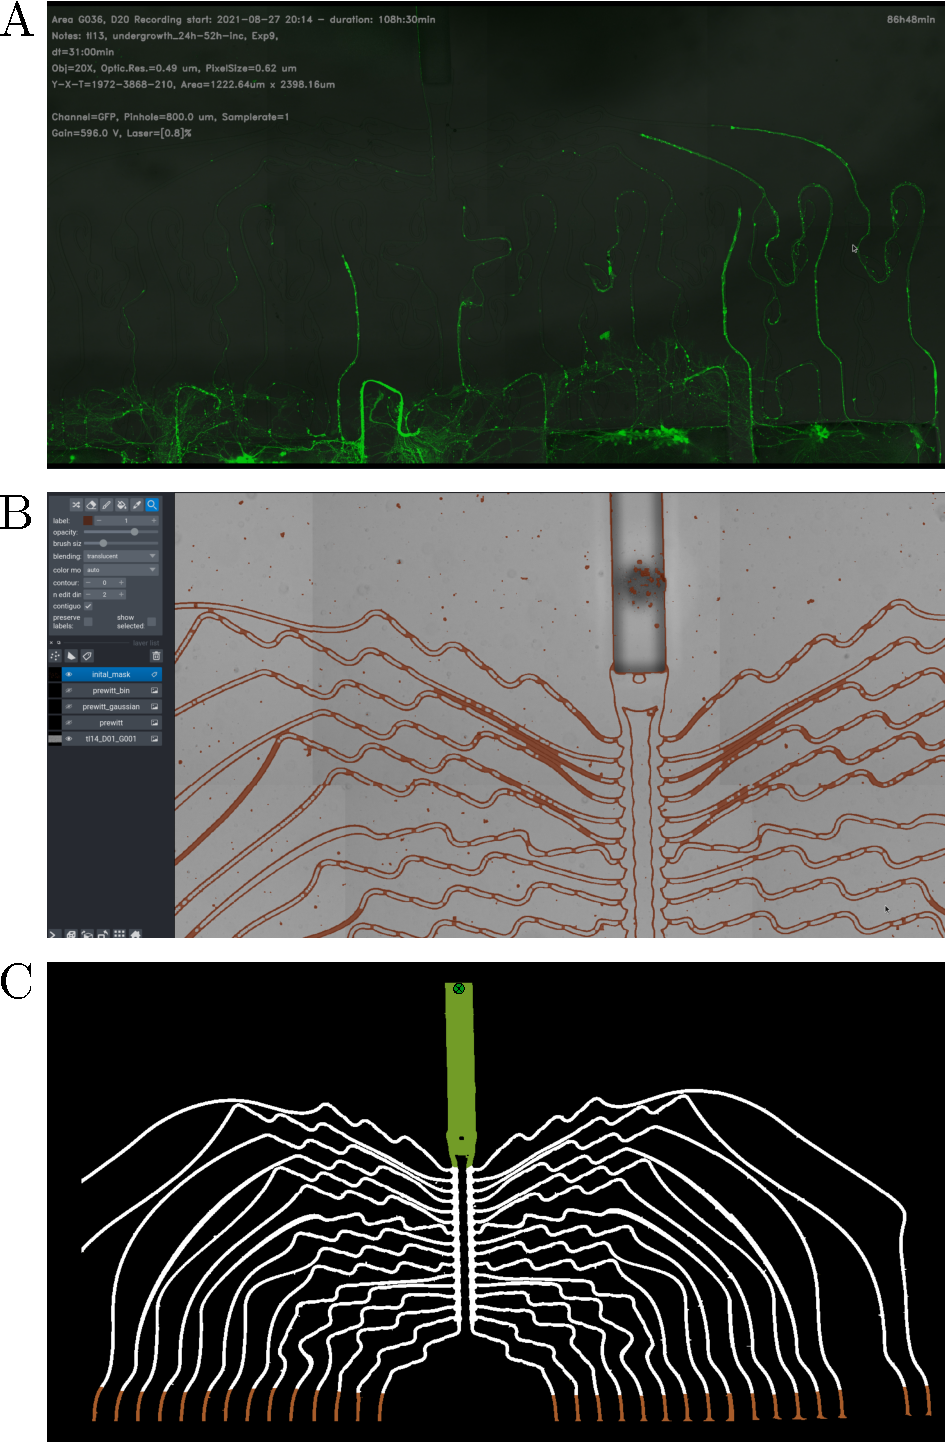
\includegraphics{SF_intial_tl_preprocessing.pdf}
    \caption[Initial timelapse preprocessing steps]{Initial timelapse
             preprocessing steps. \textbf{A} A snapshot of the exported video
             including the relevant metadata of the recording. \textbf{B} The
             napari image viewer interface with the edge segmentation layer in
             brown. \textbf{C} The manually segmented binary mask of the micro
             channels in non-black, the output channel in green, and the exiting
             channels in brown. The green dot in the output channel marks the
             target point of the PDMS design.}
    \label{SF_intial_tl_preprocessing}
\end{suppfigure}

\begin{suppfigure}[t!]
    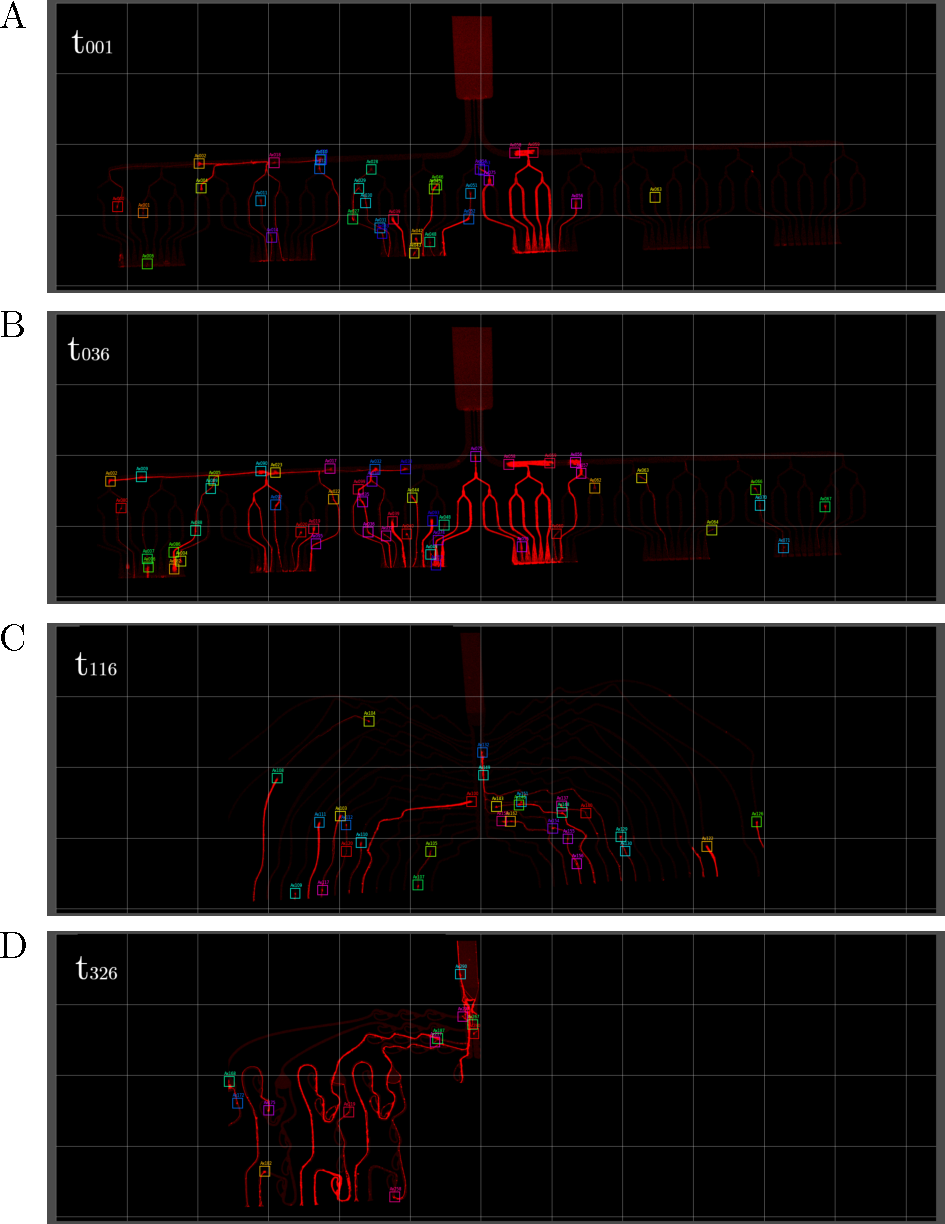
\includegraphics{SF_training_data.pdf}
    \caption[Labelled training data examples]{Labelled training data examples.
             \textbf{A} shows the first frame of the training data sequence.
             Each box represents a growth cone, the color indicates the identity
             over consecutive frames. \textbf{B} shows the last frame of
             Dataset1. \textbf{C} shows the last frame of Dataset2, PDMS micro
             structure 1 (compare Table \ref{datasets_table}). \textbf{D} shows
             the last frame of Dataset2, PDMS micro structure 2. Gridsize = 317
             $\rm\upmu m$.} 
    \label{SF_training_data}
\end{suppfigure}

\begin{suppfigure}[t!]
    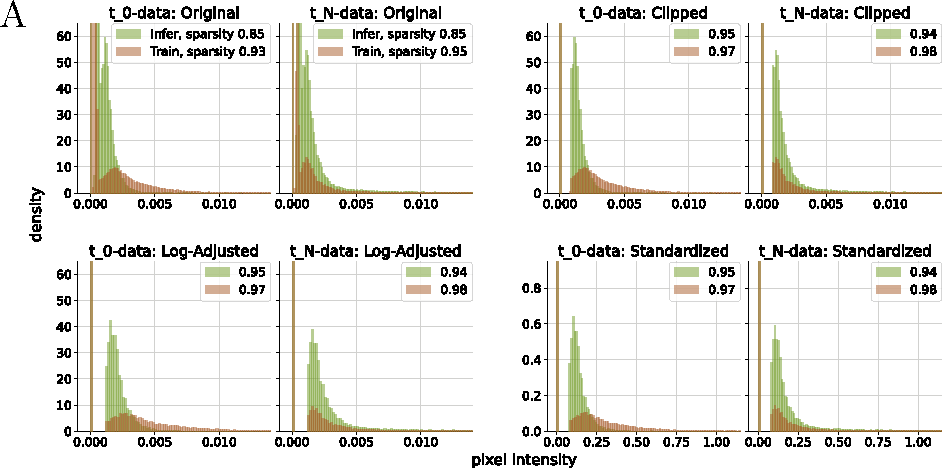
\includegraphics{SF_image_preproc.pdf}
    \caption[Preprocessing effects on pixel intensity
            distributions]{Preprocessing effects on pixel intensity
            distributions. \textbf{A} Pixel intensity distribution of training-,
            and inference data at $\rm t_0$ and $\rm t_N$ over three major
            preprocessing steps. The two plots top left show the initial pixel
            intensity distributions, top right after clipping, bottom left after
            log adjusting, and bottom right after standardization. Histograms on
            the left were obtained from sampling $10^6$ pixel values from the
            first frame, histograms on the right from the last respective frame.
            The inference data to produce the histograms (brown) was taken from
            a representative image sequence from Dataset3 (see Table
            \ref{datasets_table}). The number in the legend indicates the
            proportion of image values equal to zero (sparsity). Note that
            outlier intensity values are not shown. 
             } 
    \label{SF_image_preproc}
\end{suppfigure}

\begin{suppfigure}[t!]
    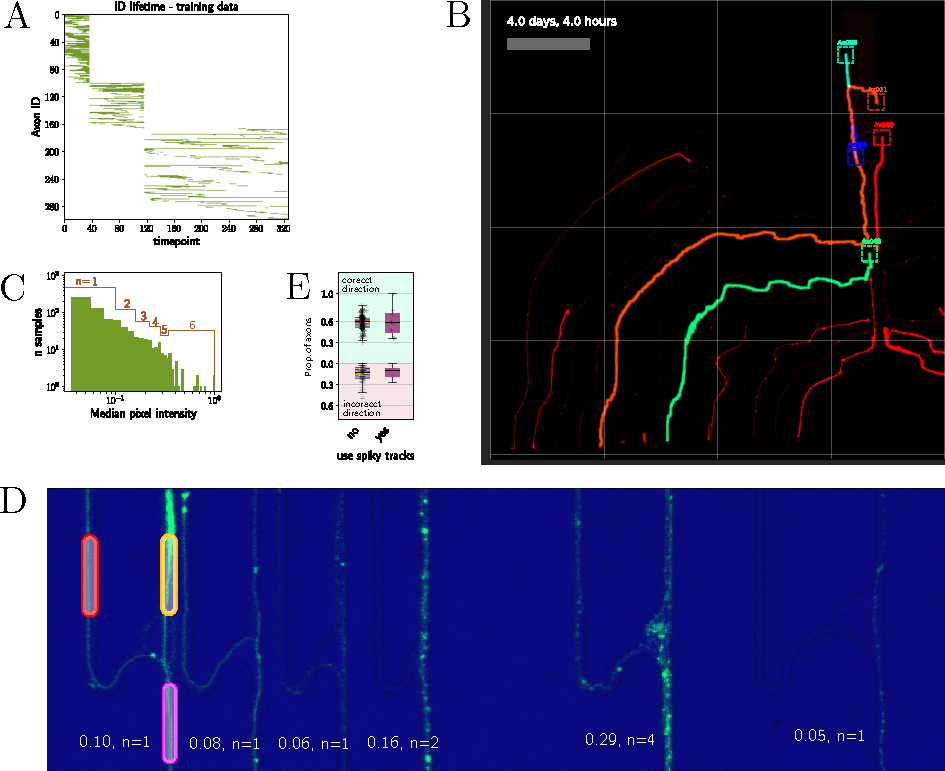
\includegraphics{SF_methods_expl.pdf}
    \caption[Methodology illustrations]{Methodology illustrations. \textbf{A}
             illustrates the axon identify lifetime. A green point on this pixel
             map indicates that a label exists for the matching axon identity
             and frame. The three clusters originate from the concatenation of
             three PDMS micro structure timelapse videos. \textbf{B} Axon
             reconstruction from growth cone track. For clarity, only a subset
             of identified axons is drawn. Gray bar width is 200 $\upmu$m.
             \textbf{C} Estimation of n axons/ duplicates (brown) from median
             intensities (green) for primitives analysis. Note double log
             scales. \textbf{D} Design primitives analysis example. Shown is the
             intermediate analysis output for the radial detachment primitive.
             The pink, yellow, and red boxes indicate the regions for computing
             inlet, biased, and unbiased median intensity, respectively.
             Annotated numbers refer to inlet median intensity and the resulting
             number of duplicates n. \textbf{E} Proportion of axons growing in
             the correct,- and incorrect direction, respectively. Split by using
             spiky tracks or not. This extends the panel from Figure
             \ref{R_directionality} D summarizing tje design features not
             significantly effecting directionality. Moved for visual clarity.}
    \label{SF_methods_expl}
    % \label{SF_labelling}
\end{suppfigure}


% \begin{suppfigure}
%     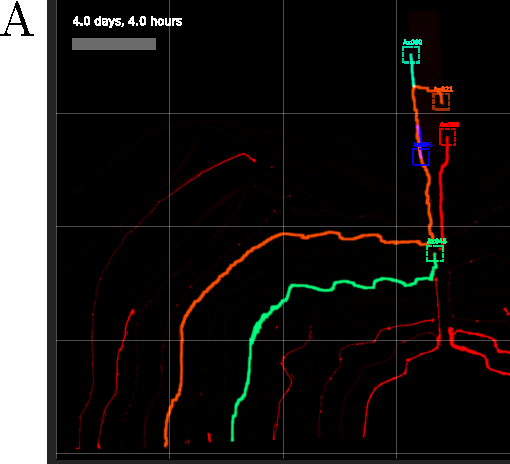
\includegraphics{SP_ax_reconstructions.pdf}
%     \caption[Axon reconstruction from growth cone track]
%     {} 
%     \label{SP_ax_reconstructions}
% \end{suppfigure}



% \begin{suppfigure}
%     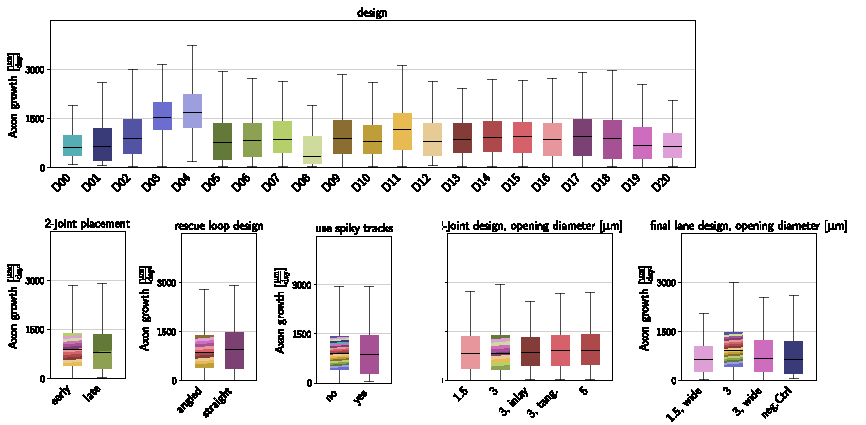
\includegraphics{SF_growthspeed.pdf}
%     \caption[Axonal growth velocity]
%     {Axonal growth velocity. Significance is not shown.} 
%     \label{SF_growthspeed}
% \end{suppfigure}


% \begin{suppfigure}
%     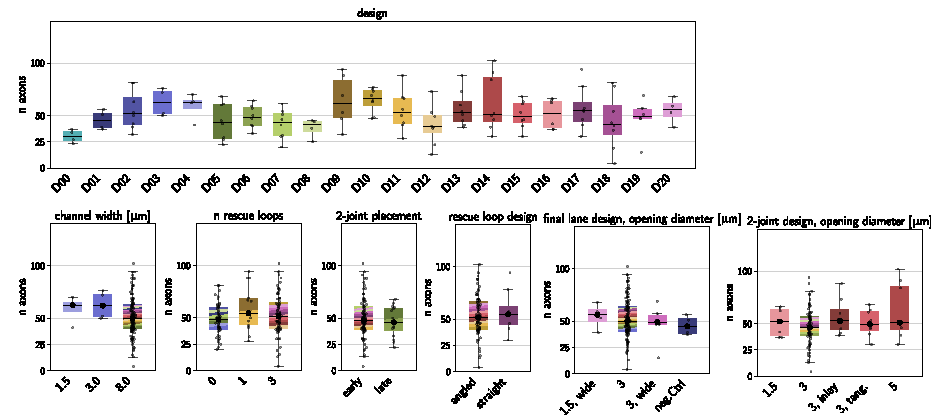
\includegraphics{SF_naxons.pdf}
%     \caption[Axon outgrowth frequency]
%     {Axon outgrowth frequency. Significance is not shown.} 
%     \label{SF_naxons}
% \end{suppfigure}


% \begin{suppfigure}
%     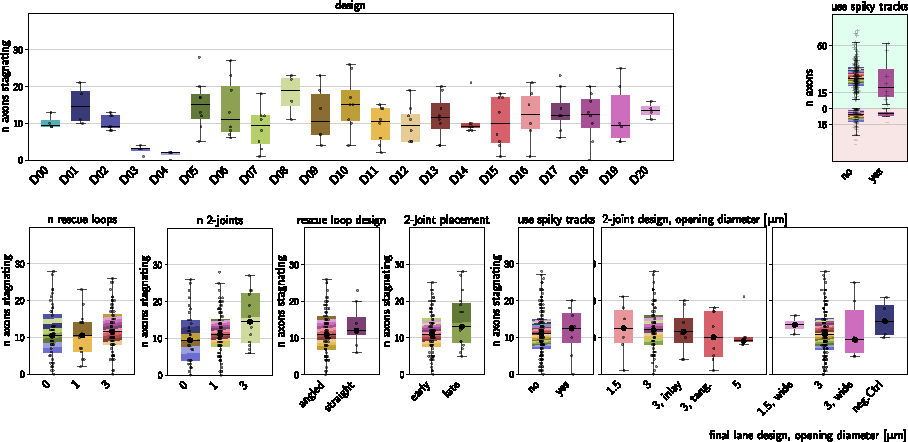
\includegraphics{SF_stagnation.pdf}
%     \caption[Number of axons stagnating]
%     {Number of axons stagnating. Significance is not shown. Top right plot shows
%     counts of axons growing incorrectly (red), and correctly (green) for a
%     feature that did not show significant effects.} 
%     \label{SF_stagnation}
% \end{suppfigure}

% \begin{suppfigure}
%     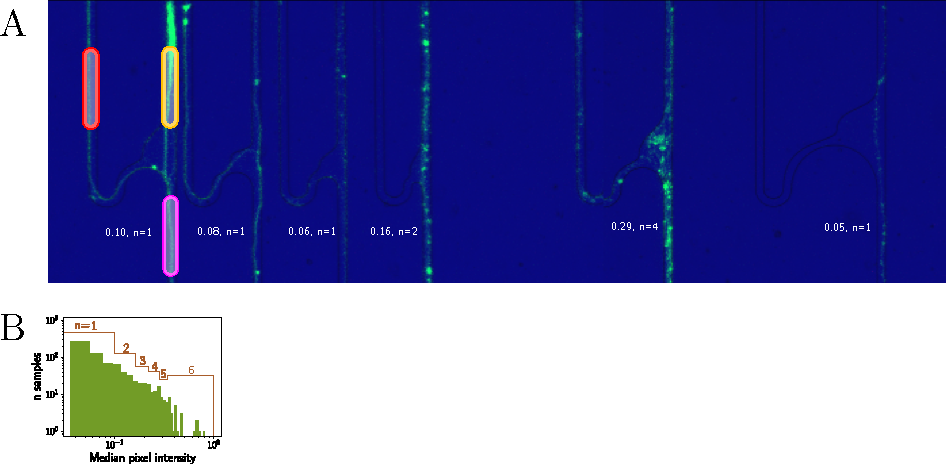
\includegraphics{SF_prim_analysis.pdf}
%     \caption[Design primitives analysis methodology]
%     {. \textbf{A} Design primitives analysis example. Shown is the intermediate
%     analysis output for the radial detachment primitive. The pink, yellow, and
%     red boxes indicate the regions for computing inlet, biased, and unbiased
%     median intensity, respectively. Annotated numbers refer to inlet median
%     intensity and the resulting number of duplicates n. } 
    
%     \label{SF_prim_analysis}
% \end{suppfigure}